\subsection{Dashboard}

Dentro del tablero “Indicadores CuCos” se crearon los siguientes indicadores:
\begin{enumerate}
    \item Cuentas Activas / Total de Cuentas – SKA1.
    \item Cuentas Activas / Total de Cuentas – SKB1.
    \item Número de cuentas con descripción en minúscula.
    \item Porcentaje cumplimiento estructura homologada – cuentas activas – SKA1.
    \begin{figure}[H]
        \centering
        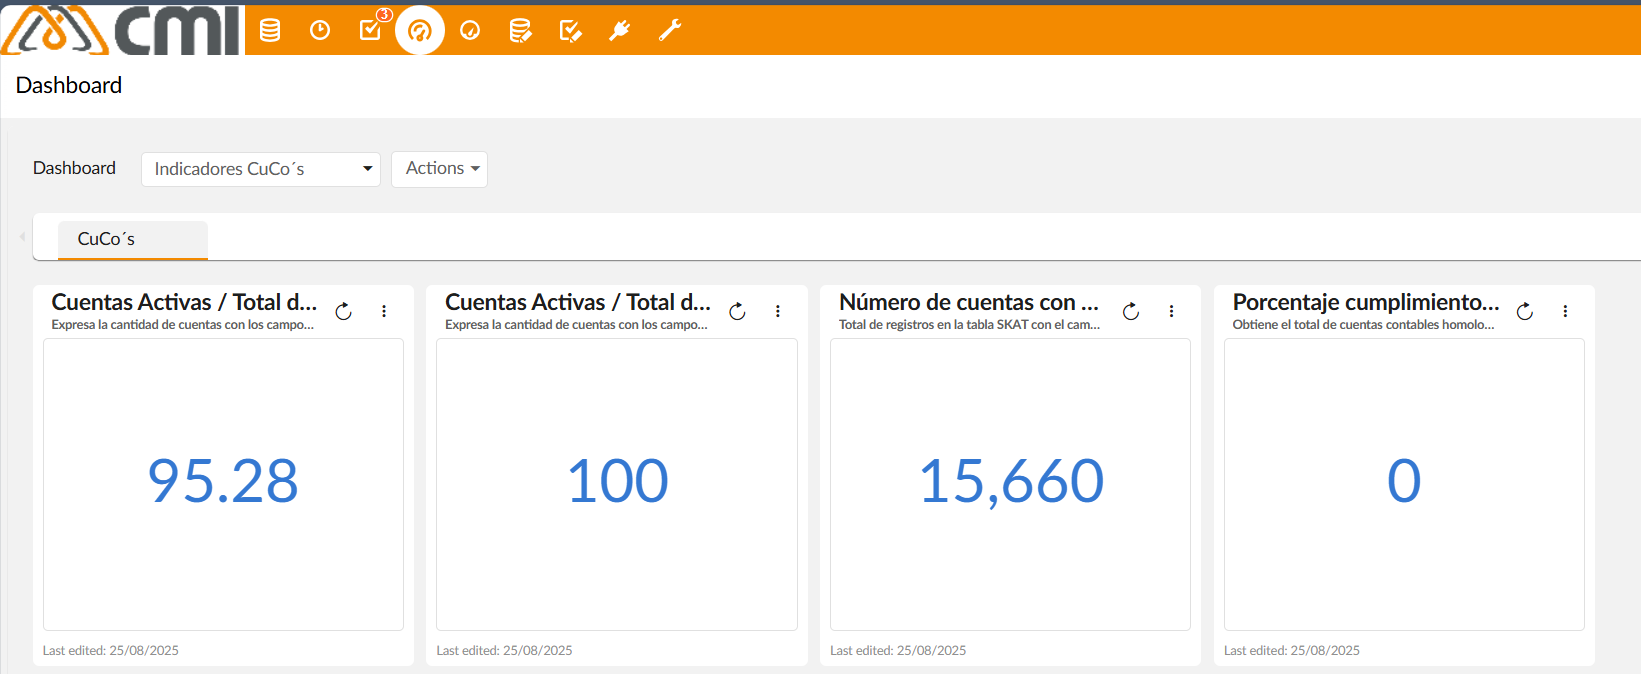
\includegraphics[width=0.8\textwidth]{WorkflowsDashboard/ImgDashboard/DB01.png}
        \caption{KPI’s mostrados en el Dashboards.}
    \end{figure}

    \item Cuentas con descripción en minúscula / Cuentas Activas.
    \item Porcentaje cumplimiento estructura homologada – cuentas activas – SKAT.
    \item Porcentaje cumplimento estructura homologada – cuentas activas – SKB1.
    \item Cuentas Activas SKA1.

    \begin{figure}[H]
        \centering
        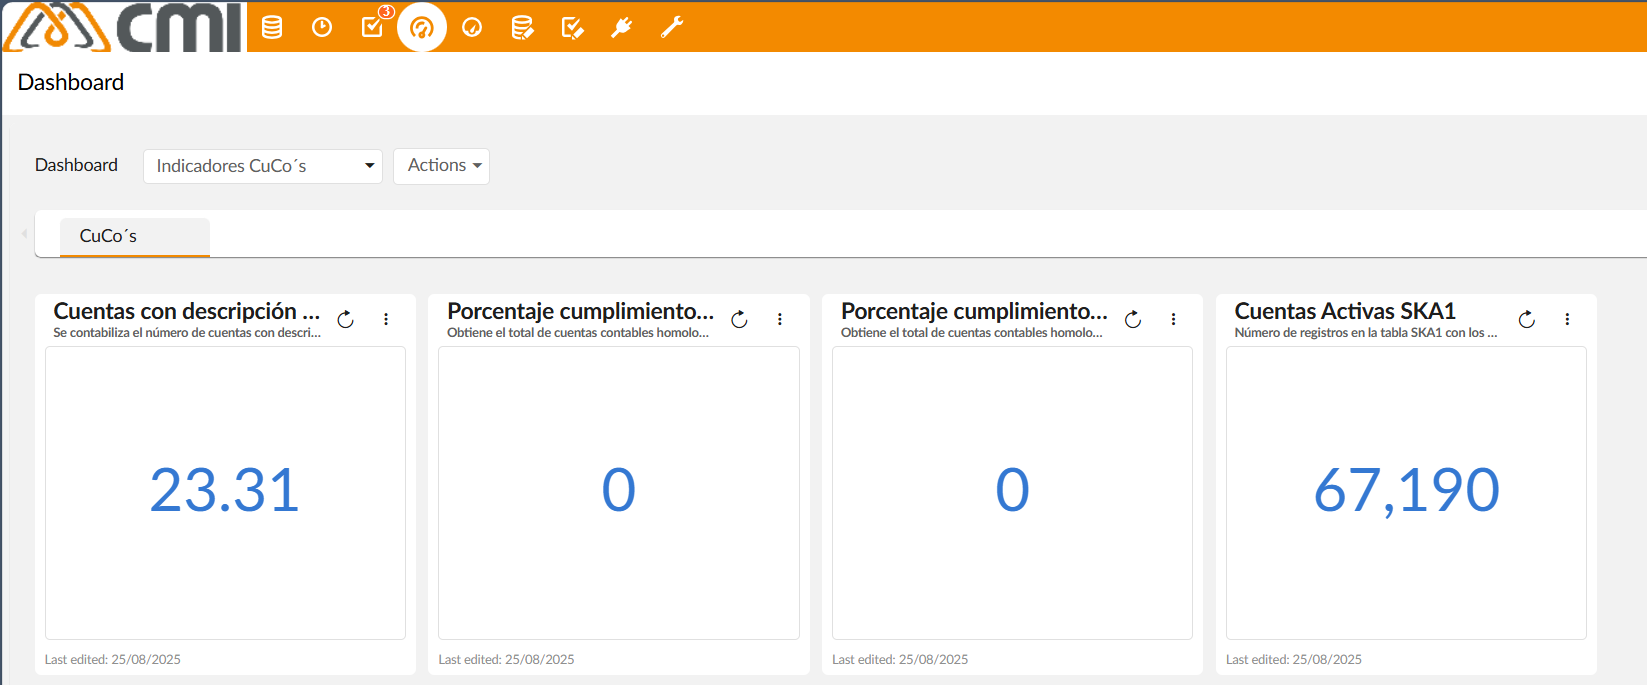
\includegraphics[width=0.8\textwidth]{WorkflowsDashboard/ImgDashboard/DB02.png}
        \caption{KPI’s mostrados en el Dashboards.}
    \end{figure}

    \item Cuentas Activas SKB1.
    \item Total de cuentas sin asignación de sociedad.
    \item Cantidad de cuentas de Resultado correctamente asignadas – SKA1.
    \item Cantidad de cuentas de activo, pasivo y capital con CECOS y CEBES asociados – SKB1.

    \begin{figure}[H]
        \centering
        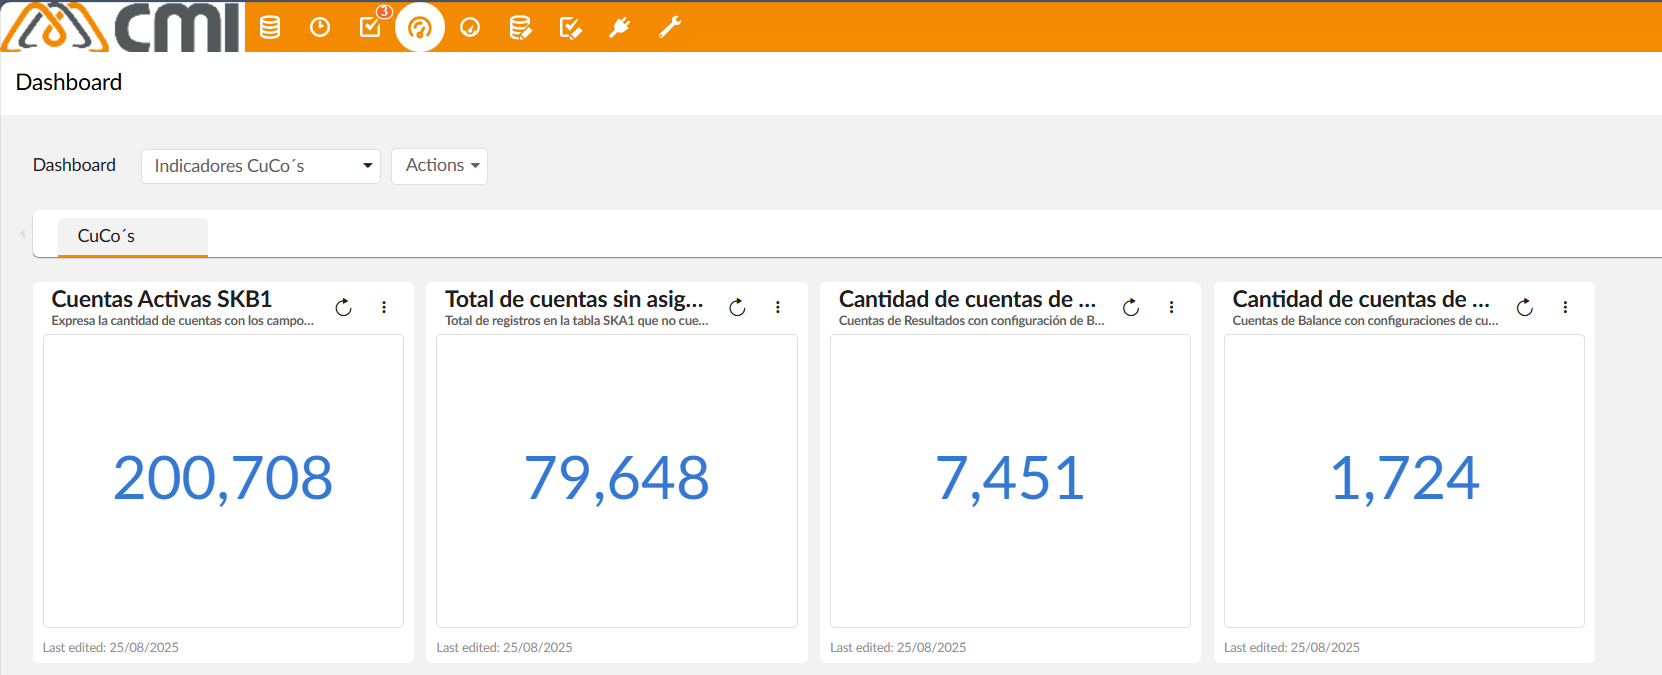
\includegraphics[width=0.8\textwidth]{WorkflowsDashboard/ImgDashboard/DB03.png}
        \caption{KPIs mostrados en el Dashboards}
    \end{figure}

    \item Cantidad de cuentas de activo, pasivo y capital con CECOS y CEBES asociados – SKA1.
    
    \begin{figure}[H]
        \centering
        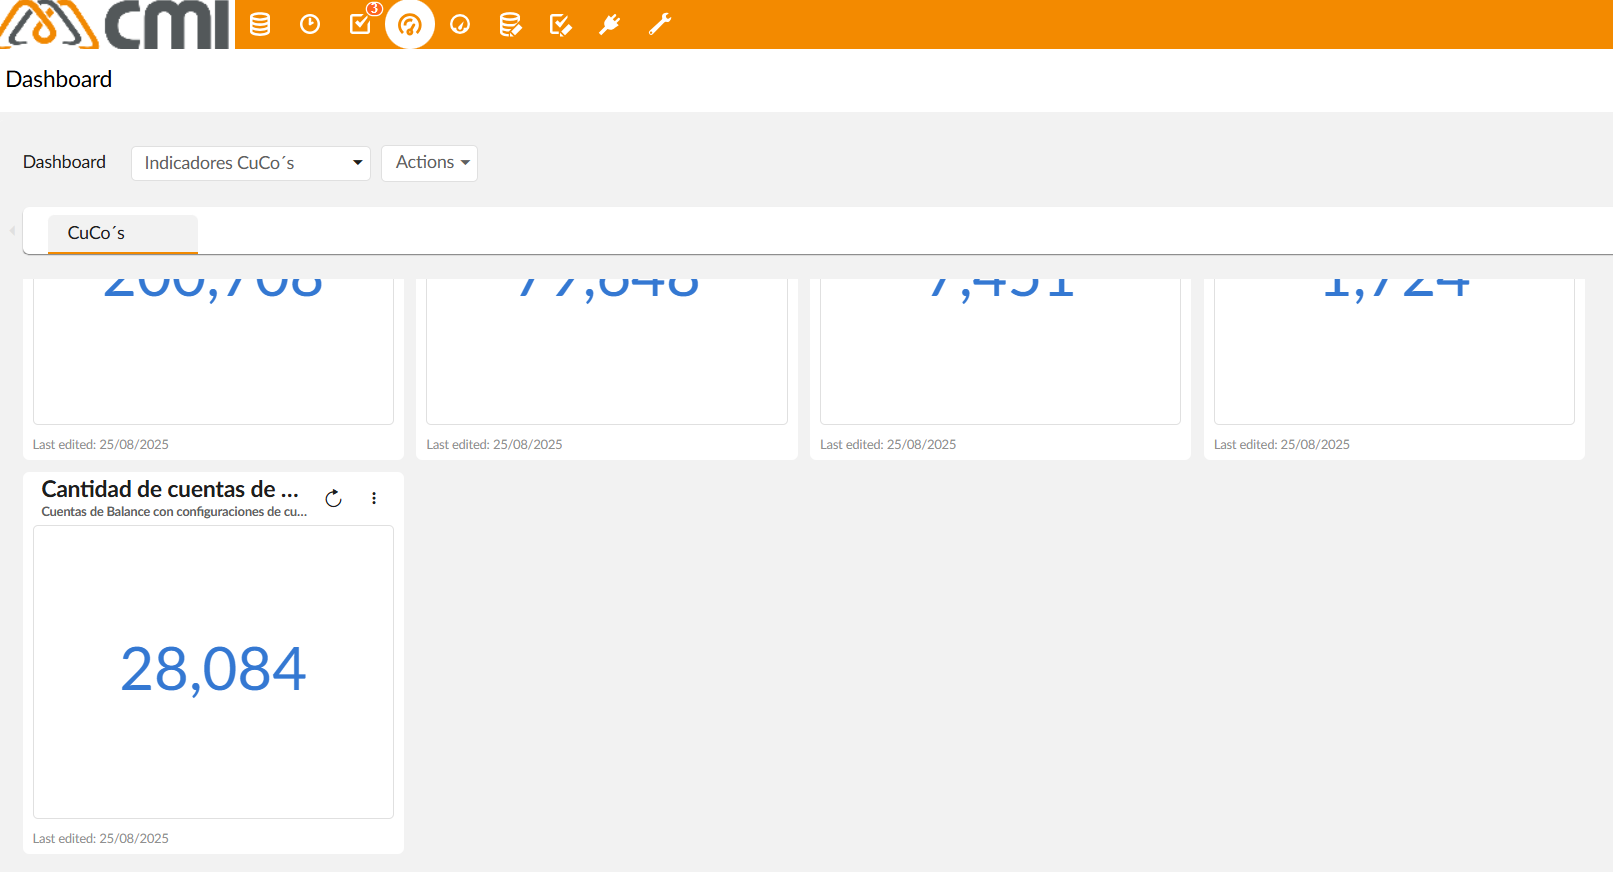
\includegraphics[width=0.8\textwidth]{WorkflowsDashboard/ImgDashboard/DB04.png}
        \caption{KPIs mostrados en el Dashboards}
    \end{figure}
\end{enumerate}







